\documentclass[conference]{IEEEtran}
\makeatletter
\def\ps@headings{%
\def\@oddhead{\mbox{}\scriptsize\rightmark \hfil \thepage}%
\def\@evenhead{\scriptsize\thepage \hfil \leftmark\mbox{}}%
\def\@oddfoot{}%
\def\@evenfoot{}}
\makeatother
\pagestyle{headings}

\IEEEoverridecommandlockouts
 \usepackage{array}
% \usepackage{algorithm2e}
% \usepackage{algorithmicx}
% \usepackage{algorithm}% http://ctan.org/pkg/algorithms
% \usepackage{algpseudocode}% http://ctan.org/pkg/algorithmicx
\usepackage{cite}

\newtheorem{mydef}{Definition}

% *** GRAPHICS RELATED PACKAGES ***
%
\ifCLASSINFOpdf
  \usepackage[pdftex]{graphicx}
\else
  \usepackage[dvips]{graphicx}
\fi


\usepackage{float}

% *** MATH PACKAGES ***
%

\usepackage{xfrac}
%\usepackage{algorithmicx}
\usepackage{algorithm}% http://ctan.org/pkg/algorithms
\usepackage{algpseudocode}% http://ctan.org/pkg/algorithmicx





\usepackage[cmex10]{amsmath}
\usepackage{amssymb}
\usepackage{xfrac}
\usepackage{xfrac}
\usepackage{color}
\usepackage[normalem]{ulem} 
\newcommand{\schange}[2]{ \sout{#1} {\color{green} #2 }}
\newcommand{\question}[1]{ {\color{red} #1 }}
\newtheorem{theorem}{Theorem}[section]
\newtheorem{lemma}[theorem]{Lemma}
\usepackage[caption=false,font=footnotesize]{subfig}
\usepackage{url}
% \usepackage{hyperref}
\hyphenation{op-tical net-works semi-conduc-tor}

\newcommand*{\PROB}{\mathbf{P}}

%%versions
% \usepackage{versions}
% \includeversion{conf}
% \excludeversion{extended}

%  \includeversion{extended}
%  \excludeversion{conf}


\begin{document}
\title{Detection Mechanism for Internal Attacks on Pull-based P2P Video Streaming Systems}

% \author{\IEEEauthorblockN{Hatem Ismail}
% \IEEEauthorblockA{DEEDS Group, TU Darmstadt\\
% % Darmstadt, Germany\\
% hayman@deeds.informatik.tu-darmstadt.de}
% \and
% \IEEEauthorblockN{Stefanie Roos}
% \IEEEauthorblockA{University of Waterloo \\
% % Waterloo, Canada\\
% stefanie.roos@uwaterloo.ca}
% \and
% \IEEEauthorblockN{Giang Nguyen}
% \IEEEauthorblockA{TU Dresden\\
% % Darmstadt, Germany\\
% giang.nguyen@tu-dresden.de}
% \and
% \IEEEauthorblockN{Neeraj Suri}
% \IEEEauthorblockA{DEEDS Group, TU Darmstadt\\
% % Darmstadt, Germany\\
% suri@cs.tu-darmstadt.de}
% }


% make the title area
\maketitle

\begin{abstract}

Video streaming is a very popular service and P2P-based solutions for streaming can reduce costs for both providers and users.
Yet, involving users into the data dissemination entails security risks including a variety of denial-of-service attacks. 
While extensive research exists on mitigating varied attack types, the class of inference attacks (where the attacker is capable of inferring the peers directly connected to the source), still constitutes a major open threat for streaming P2P systems.

Our research focuses on the critical class internal inference attacks for pull-based overlays, where the attacker first infers the overlay's topology before conducting a buffer-map ($BM$) cheating attack using malicious peers located at the positions closest to the source. 
We demonstrate the feasibility of conducting such attacks, and also show how very few malicious peers can drastically compromise the P2P overlay.

Accordingly, we propose a two-fold detection mechanism that is capable of (a) detecting the malicious peers conducting various\mn[Stef]{Are we still doing 'various'? I would say only dropping} $BM$ cheating behaviors in the worst case scenario where 100\% of the sources neighbors are malicious\mn[Stef]{detecting the worst-case attack is not really an achievement, detecting less obvious attacks is... I would rewrite this}, and (b) restoring the the overlay to a benign state.\mn[Stef]{What is a `benign state'? sounds like we actually remove nodes} 
The proposed mechanism allows peers to collaboratively detect and notify the source, which in turn replaces the suspected peers.

% Simultaneously, peers locally sanitize their contact lists from peers who conduct adversarial $BM$ cheating behaviors.

Using a combined theoretical and simulation-based analysis, we validate that the detection mechanism is able to detect malicious peers with up to 80-90\% accuracy while inducing a small overhead of  approximately 8\%. Furthermore, we ascertain theoretically and hrough simulations that malicious peers cannot misuse the detection mechanism to gain influence. 

\end{abstract} 
\section{Introduction}
\label{sec:intro}

Streaming content is an essential component of data-driven infrastructures \cite{emule}.
Most streaming applications rely on (monopolistic) central providers that have significant computing and communication resources to distribute high quality of service content to a large audience in a fast and reliable manner. For the providers, this entails the use of dedicated resources, involves performance and scalability issues along with considerations of handling single point of failures.
Distributing content via a Peer-to-Peer (P2P) network significantly lowers the load that the provider experiences as the participants relay the downloaded content to other participants. This eliminates the need that all participants receive their content directly from the source, i.e., the provider. 
Consequentially, P2P streaming (including P2P streaming into the service of established providers) becomes an attractive option for alternative distributed providers and user-generated content to help reduce data delivery costs and resultant lower rates for customers.


However, achieving high reliability in a P2P overlay and across a dynamic and heterogeneous group of content distributors is challenging. In addition to the inherent operational unreliability of benign participants, attackers such as competitors can infiltrate the set of peers and conduct denial-of-service attacks. In this manner, malicious participants can interrupt or delay the distribution of the content with the goal of degrading the quality of service. 

In general, nodes in a P2P streaming system connect to a small set of other nodes, called the \emph{neighbor set}. 
The publisher or the \emph{source} of the content divides the stream into \emph{chunks}, which each contain an equal-sized part of the encoded data, and forwards these chunks to its neighbors. Nodes in the system receive chunks from neighbors and forward them to neighbors that have not previously received the respective chunks. 
The selection of neighbors and the choice of neighbors to receive-from or forward-to differs across protocols \cite{sasi2014survey}.  Yet, pull-based mesh networks are the predominant method in P2P streaming systems \cite{zhang2014modeling}. In a mesh overlay, peers maintain a buffer-map indicating which chunks they possess.  Neighbors periodically exchange their buffer-maps and request chunks from neighbors whose buffer-maps indicate possession of the respective chunk. Peers then forward chunks based on the received requests. 


In pull-based systems, there exist several denial-of-service attacks, known as buffer-map or $BM$ cheating attacks \cite{cheatingAnalysis}. 
In such an attack, malicious nodes might drop or delay chunks. Alternatively, they might advertise chunks that they do not have. As detection of the latter is locally possible and the effect of delaying chunks is at most as severe as entirely dropping the respective chunks, we focus on a denial-of-service attack through dropping chunks without advertising them, called \drop in the following.  


In the past, multiple countermeasures aimed to reduce the severity of the \drop attack. However, the majority of these defences \cite{zhang2005coolstreaming, defending2, antiliar} assume that the attacker is unaware of the topology of the streaming network and specifically does not know the \emph{headnodes}, i.e., the peers connected to the source. 
However, previous work indicates that it is relatively easy to infer the identity of benign headnodes and then target those important nodes \cite{nguyen2016swap}.
While countermeasures to these inference attacks exist, they assume an external adversary that can shut-down or replace certain nodes \cite{nguyen2016swap, rbcs, nguyen2014resilience}. 
Hence, the existing work evaluates neither the impact of nor protection mechanism against internal colluding attackers, i.e., attackers that insert nodes under their control into the system pretending to be regular participants. 


In this paper, we first illustrate the effectiveness of internal attacks based on malicious headnodes. 
Consequently, we propose a mechanism for detecting \drop by keeping track of peer satisfaction. If the cumulative satisfaction level of a group of peers drops below a certain threshold, the source replaces all headnodes associated with the group with randomly chosen peers. 
Hence, our detection and mitigation mechanism efficiently reacts to a detected low quality of service.
Note that we focus on attackers that control a low fraction of nodes, as attackers controlling the majority of nodes can trivially control most of the communication, even without gaining strategically important positions such as headnodes.    

Using a simulation study, we show that the proposed detection mechanism can fully restore peers satisfaction, even in a scenario where the attacker controls all headnodes. 
Our mechanism introduces only a small signaling overhead of approximately $8\%$ supporting the claim of being both effective and efficient.

A theoretical analysis complements our practical results, focusing on the opportunities to abuse the detection mechanism. 
Indeed, the detection algorithm prevents malicious nodes from replacing benign headnodes with malicious nodes unless they control a large fraction of the total number of nodes. 
Furthermore, maintaining malicious headnodes despite generally low satisfaction levels is not possible for the considered attacker. 
  
% 
% at detection malicious behaviors in a fast, low overhead approach while considering the case where the attacker can fully occupy the source's neighbor list with malicious headnodes.
% In details, peers are able to trigger a request to their neighbors once (a) a peer is, with evidence, performing maliciously, or (b) generally, the stream satisfaction (the user's experience) of a peer drops below a given application threshold.
% Once proven malicious, a peer fires a complaint, on behalf of all other participants in the detection process, to the source to remove the detected peer from it's neighbor list,
% or to generally decide about peers that might be affecting the satisfaction level of non-headnodes.
% \subsection*{Paper Structure}
% \mn[Stef]{I dislike paper structure sections, but that is personal taste; I can deal with them by ignoring them, which is what I did with this one}
% The rest of the paper is organized as follows: Section~\ref{sec:related} discusses the related work and the background.
% In Section~\ref{sec:Attack}, the concepts underlying the attacker model internal attack and the conducted adversarial behaviors are defined.
% The detection mechanism is fully discussed in Section~\ref{sec:detection}, with the theoretical analysis is discussed in Section~\ref{sec:analysis}.
% The internal attack's impact, along with the detection mechanism performance and efficiency, are evaluated in Section~\ref{sec:eval}. Finally, we conclude our work and discuss the future work in Section~\ref{sec:conclusion}.

\section{Related Work}
\label{sec:related}

We overview the prominent existing work on attacks and their detection in the context of P2P streaming systems. Most prior work has considered three attack types: (i) pollution attacks, i.e., flooding the overlay with arbitrary content and claiming it to be relevant chunks, (ii) free riding, i.e., participating in the overlay without contributing, and iii) cheating attacks, i.e., maliciously dropping packets or manipulating buffer-maps. 

Pollution attacks are one of the most common attacks \cite{pollution1}. Strategies such as network coding \cite{nc} and others \cite{pollution2} 
can effectively mitigate these attacks. 

In contrast, the main approach to counter free riding are incentives \cite{defending,defending2}, i.e., rewarding peers that distribute the stream to others. 
However, these strategies are only effective for peers that aim to minimize their level of participating. 

  
Cheating attacks are severe DoS attacks, performed to maximize the damage to the overlay and preventing peers from downloading the stream.   
\textit{Antiliar} is a general defense mechanism against a diverse set of attacks, including dropping and buffer map manipulation\cite{antiliar}.
Mainly, \textit{Antiliar} tracks peers behaviors in a secure progress log and thus, detecting misbehaving peers by identifying irregularities in the log. 
While highly effective, \textit{Antiliar} relies on expensive cryptographic operations that are unsuitable for devices with low CPU resources.
Moreover, \textit{Antiliar} uses a central entity to review the logs, creating additional security and privacy problems. 


An alternative  decentralized approach \cite{nguyen2014resilience} relies on redundancy by enforcing diversity when requesting chunks. 
In this manner, the attacker has to control a higher fraction of nodes to achieve any severe damage by cheating.
The work focuses in particular on attacks on headnodes yet assumes an external attacker that can take over arbitrary nodes at will.
In this context, the idea of swapping headnodes frequently to mitigate the impact of the attacker's control can significantly decrease the attack severity \cite{nguyen2016swap}.
As shown in Section~\ref{sec:eval}, internal attackers can undermine the swapping protocol and gain the position of headnodes.  

% \section{System Model}
\label{sec:system-model}

\section{Internal Attack Model}
\label{sec:Attack}

In this section, we introduce the concept of internal attacks in the context of streaming P2P overlays.
Our focus are attacks on availability that aim to intercept video chunks from the source. 
We start by introducing attack characteristics such as target, budget, and placement of malicious nodes. 
Afterwards, our main discussion outlines the the various adversarial behaviors that can be applied by a malicious peer once a video chunk has been intercepted. 

\subsection{Target, budget and placement}


The target of the internal attack is to severely degrade the user's satisfaction by interrupting the video stream close to the source, thus preventing dissemination between benign peers.
Accordingly, the attacker aims at using its budget to occupy the source's neighbor list, where budget denotes the malicious peers $m\in M$ the attacker can place in the system.
Note that in a real streaming system, the typical size of the source's neighbor list is 20-30 entries \cite{neighborlist1,neighborlist2}, which highlights the feasibility of conducting the internal attack using a very small budget.

Assume an attacker with budget $x$ is capable of assigning malicious peers as headnodes.
In fact, it is feasible to do so, for example through (a) joining the overlay as early as possible in case of a pre-announced time for a streamline, (b) taking down the source's benign headnodes, or (c) Abusing peers' replacement mechanisms \cite{nguyen2016swap}.
Hence, the attacker initially assigns a fraction $\eta x$, where $\eta\in [0,1]$, of its resources as headnodes.
As the attacker's main objective is to fully occupy the source's neighbor list, the optimum value of $\eta$, from the attacker's perspective, is when $\eta x = |NeighborList|$.
In case such full exploitation of the source's neighbor list is not feasible when the attack is being initiated, the attacker continuously tries to increase the value of $\eta$.  

The rest of malicious peers $MN=x-\eta x$ are assigned as neighbors to the $\eta x$ malicious headnodes, i.e., those peers are not headnodes, they are connected as neighbors to the malicious headnodes. 
Nonetheless, such placement is considered the best strategy for the attacker for the following reasons: (a) $MN$ is used to counter headnodes replacement mechanisms such as SWAP \cite{nguyen2016swap}, i.e., malicious headnodes $\eta x$ keep on advertising $MN$ to the source for swapping, and thus, $MN$ are promoted as headnodes
, and (b) as benign peers in malicious headnodes neighbors 


Given the fact that inferring the overlay's topology is indeed feasible \cite{nguyen2016swap,rbcs}, accordingly, the attacker is capable of inferring the existing headnodes in the system.
Accordingly, such distribution of the attacker's budget assures that even if the attacker is not able to directly place malicious peers as the source's neighbors (headnodes), having a higher budget to occupy the headnodes' neighbor lists also results on a complete shut down of the stream from the rest of the overlay.

\subsection{Adversarial behaviors}
Here we discuss three basic adversarial behaviors that are executed either simultaneously with a certain probability or standalone according to the attacker's target, budget and the susceptibility to being detected.
In Section~\ref{sec:eval}, we provide a simulation study to demonstrate the impact of the different attack scenarios below.

\subsubsection*{Dropping behavior}
When a malicious peer $m$ receives a video-chunk from the source or even through another headnode, $m$ drops the packet. 
Hence, $m$ never advertises for those chunks and instead, keeps on requesting the dropped chunks from other benign peers $b \in B$.
This scenario guarantees that: (a) malicious peers are less susceptible to being suspected given that the requesting benign peers are not aware that $m$ indeed received those chunks,
and (b) are incapable of inferring that the malicious headnodes fraction $\eta x$ is an actual headnode as the availability and the freshness of chunks in the buffer-maps are a key factor to infer the position of a peer.
>>>>>>> f3f7cad3b0f1f2cc09cb46e99a7c83d2b29159a7

\subsubsection*{Manipulating behavior}
When executing manipulating behavior, $m$ sends its updated buffer-map to $b$, i.e., it advertises received chunks. 
Although having the actual video chunks $m$ advertised for, $m$ never sends the requested video chunks from $b$.
In this scenario, malicious peers are more susceptible to being detected, however, a benign peer might be overloaded and can not serve all the requests it receive and might also appear manipulating to other benign peers.
In Section~\ref{sec:detection}, we further discuss this case and propose a procedure that decreases the likelihood of suspecting a benign peer of being malicious.

\subsubsection*{Outdated time stamps behavior}
In this behavior, $m$ simply advertises for the chunks in its buffer-map. 
However, $m$ starts serving the requests once the requested chunks are considered out-dated.
Similar to the manipulating behavior, malicious peers are more susceptible to being detected than in the dropping behavior case.





\section{Detection Mechanism}
\label{sec:detection}


In this section, we explain our detection mechanism, starting with an overview of the different steps followed by a detailed description of each step.  
The goal of the detection algorithm is to restore the user's satisfaction in the face of a \drop attack. The key idea of our method is to replace headnodes associated with peer groups of low satisfaction levels. 

Throughout the section, we assume that nodes authenticate their messages using digital signatures. 
% Hatem: trim
% The source keeps track of the verification keys of all participants and can hence establish the authenticity of messages.
The source keeps track of participants' verification keys and can hence establish the authenticity of messages.
In particular, malicious nodes cannot forge responses of honest peers to influence the mechanism. 
We assume that neighboring nodes periodically exchange messages stating that they are neighbors.
These \emph{proofs of neighborhood} are signed and contain a time stamp. 
In this manner, $u$ can proof if $v$ is (or has recently been) its neighbor. 





\subsection{Mechanism Overview}
We illustrate the underlying ideas of the detection mechanism in Figure~\ref{detection-blocks}.
When a malicious peer $m$ performs a \drop attack, benign peers $b$ are unable to immediately identify the malicious behavior.
Specifically, $m$ never sends the actual $BM$ that represents the chunks it currently possesses, i.e., $m$ is only requesting chunks it already has. 
Thus, detecting a violation in this case is not straight-forward. In particular, nodes are generally unable to identify a suspected attacker based only on local information.
In the remainder of the section, we present a mechanism that allows nodes to collaboratively identify suspects that are subsequently removed as headnodes.  




\begin{figure}
 \centering
 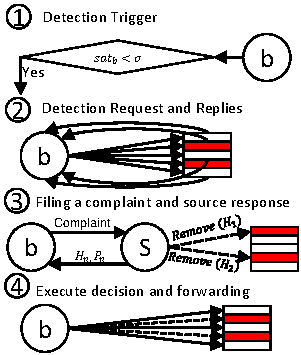
\includegraphics[width=5.5cm,height=6.5cm]{./Figures/detection.pdf}
 
  \caption{Detection process for \drop. $S$ denotes the source.}
   \vspace{-3.5mm}
\label{detection-blocks} 
\end{figure}



The detection consists of four steps, starting with an initial trigger of dissatisfaction at one peer and potentially terminating in replacing one or several headnodes. 
First, when a peer $b$ suspects a \drop attack based on its local observations, $b$ sends a \emph{detection request} to all peers in its neighbor list.
Second, each peer receiving a detection request prepares a response. 
Third, the initiator $b$ decides based on the received responses if they should file a complaint to the source. 
If $b$ decides to file the complaint, $b$ sends it on behalf of the participating peers in the request. 
Afterwards, the source verifies the complaint, reacts accordingly, and responds to $b$, detailing the steps taken. 
The reaction of the source is either the replacement of one or several headnodes or the rejection of the removal request.
Finally, $b$ reacts based on the received response from the source and then forwards the source's reply to the other participants in the complaint, who in turn execute the same procedure.

The node $b$ bases its decision on whether to initiate a request or forward a complaint on a number of threshold parameters, which we summarize in Table~\ref{tab:acronyms} together with various system parameters governing the attack. 

\begin{table}[ht]
\center
\caption{Acronyms}
\begin{tabular}{|c|l||c|l|}
\hline

\bf{Var.} & \bf{Description}  & \bf{Var.} & \bf{Description} \\\hline\hline
$H_n$ & headnodes in a complaint & $P_n$ & potential candidates list \\\hline
$x$ & no. of malicious peers & $\eta$ & mal. headnodes fraction\\\hline
$BM$ & buffer-map & $MN$ & mal. non-headnodes \\\hline
$\sat$ & peer satisfaction level & $\satThres$ & satisfaction threshold \\\hline
$\minP$ & min. drop responses & $\minDR$ & no. allowed det. \\\hline
\end{tabular}
\label{tab:acronyms}
% \vspace{-3mm}
\end{table}

\subsection{Detection Trigger}
\label{Detection-Trigger}


In order to start a detection request, the node $b$ has to experience a low satisfaction level. 
The satisfaction of a peer is defined as the fraction of missed chunks, i.e., the continuity of the stream according to the $Hit/Hit+miss$ chunk ratio.
% \mn[Stef]{how many chunks does the peer consider for that; all during the whole download, only the last $s$ seconds?}
In a nutshell, $b$ starts a detection request if its satisfaction is below a satisfaction threshold $\satThres$.
However, to limit the ability of malicious peers to incorrectly accuse benign peers and increase the load through false detection requests, the concrete conditions that result in a detection request from $b$ are: 

% \begin{itemize}[noitemsep,wide=0pt, leftmargin=\dimexpr\labelwidth + 2\labelsep\relax]

\begin{enumerate}
% \begin{compactenum}
 \item $b$'s current satisfaction level $\sat_b$ is less than the predefined threshold, i.e., $\sat_b < \satThres$.
 \item The number of drop detection requests sent by $b$ in the time interval $t_{det}$ is less than $\kappa$. 
 \item $b$ has not initiated or replied to any other \drop detection request that the source has not decided on yet.
% \end{compactenum}
\end{enumerate}
The second and third condition guarantee that peers cannot abuse the mechanism via triggering or participating in multiple detection requests in parallel. 
Moreover, restricting concurrent requests for benign peers is sensible as their low satisfaction level is already noted in their reply to previous requests.

\subsection{Processing a Detection Request}
Let $D$ denote the set of queried peers, i.e., the neighbors of the initiator $b$ if $b$ executes the protocol honestly.  
When receiving a detection request, a peer $d \in D$ hence first checks if it can participate in any more requests.     
If so, $d$ replies with its $\sat_d$ and a time stamp, both signed by its private signature key. 
The time stamp prevents the attacker from replaying benign peers' previous (low) satisfaction levels, as only recent satisfaction levels are valid.


\subsection{Filing and Processing a Complaint}

Upon receiving a feedback from its neighbors, $b$ decides whether to file a complaint or not.
If so, the source verifies the complaint and potentially removes some of its headnodes. 

\subsubsection*{Filing a complaint}
$b$ will start processing the replies once all nodes in $D$ have replied or a time-out $t_{replies}$ occurs. 
We assume that the source's address is publicly known and $b$ can send a complaint to the source directly.

$b$ sends a complaint if the average satisfaction level indicated in the responses is below a threshold $\satThres$ and at least $\minP$ peers replied to the request. 
More specifically, let $\sat_1, \ldots ,\sat_z$ be the satisfaction levels expressed in the replies and $\sat_b$ be $b$'s satisfaction level. 
Assuming a sufficient number of replies, $b$ files a complaint to the source if:
\begin{align}
\label{eq:drop_satis_equation}
\frac{1}{z+1}\left( \sat_b + \sum_{i=1}^{z} \sat_i \right) < \satThres. 
\end{align} 
Otherwise, $b$ either starts another detection request depending on $\kappa$ or waits until allowed to send another detection request.
 

Once $b$ decides on filing a complaint according to the aforementioned conditions, $b$ generates a complaint message to the source containing the IDs of all nodes in $D$, recent proofs of neighborhood,  and the received satisfaction levels including signatures and time stamps.  


The reason for requesting at least $\minP$ replies is to prevent a few malicious nodes from accusing benign headnodes. By imposing a lower bound on the requested number of replies, a considerable number of malicious nodes has to use one of their $\kappa$ requests. We present an in-depth analysis on how these constraints prevent misuse in Section~\ref{sec:analysis}. 

\subsubsection*{Processing a Complaint at the Source}

The source $s$ first verifies the content of the complaint. First, the source rejects any complaint from a node $b$ that has already participated in $\kappa$ requests. 
If $s$ does not reject the complaint, $s$ then removes any satisfaction levels without valid signatures from the complaint.
Furthermore, $s$ removes any responses from nodes that have exceeded their participation limit or are participating in two complaints at the same time. 

If the remaining valid responses still indicate an average satisfaction level of less than $\satThres$, the source:  
\begin{enumerate}
 \item divides the set of peers in $D$ into two sets $H_n$ and $P_n$, where $H_n$ is the set of headnodes peers that exist in the complaint. 
%  \mn[Stef]{Itemize lists are strange as they are not full sentences but start with a capital letter and end in .}
 \item removes all peers in $H_n$ from its neighbor set.
 \item randomly connects to another $|H_n|$ peers. 
 \item adds peers (excluding peers in $H_n$) from its neighbor list to $P_n$, where $P_n = NeighborList\setminus H_n$ ($NeighborList$ is the set of peers in a neighbor list). 
 \item sends a \textit{Complaint Reply} to $b$ containing $H_n$ and $P_n$.
\end{enumerate}
 The reason for choosing random new headnodes rather than nodes participating in the complaint is to lower the incentive for complaints by malicious peers.
 Even if such a complaint is successful, the new headnodes are likely benign, meaning that the malicious nodes did not gain anything from initiating the request apart from slightly increasing the load. 


\subsubsection*{Processing a Complaint Reply \& Forwarding}

Finally, when $b$ receives the \textit{complaint Reply} from the source, $b$ 
\begin{enumerate}
 \item Disconnects from all peers in $H_n$. Note that $b$ does not blacklist peers in $H_n$ from its neighbor list due to the fact that those peers are not proven malicious.
 \item Connects to $|H_n|$ peers from $P_n$, in case $|H_n|>|P_n|$, peers connect to $|P_n|+(|H_n|-|P_n|)$ random peers.
\end{enumerate}
Subsequently, $b$ forwards the complaint to the other participants, i.e., $D \setminus H_n$, who in turn execute steps 1 and 2.

\subsection{General Notes}
The detection mechanism does not aim at expelling peers from the system. Simply removing headnodes remarkably benefit the system.
Indeed, the only peers that get blacklisted are those who violate the detection mechanism constraints, i.e., participating in more than a single request at a time or initiating more than $\kappa$ requests.
The reason for this leniency lies in the potentially high chance of removing headnodes that are benign but exhibit a low performance. 
In general, the main target of the detection mechanism is to enhance peers' satisfaction level while keeping peer replacements and signaling overhead low. 







\section{Analysis}
\label{sec:analysis}


We focus on characterizing the behavior of malicious nodes aiming to subvert the detection mechanism to remove honest headnodes and retain malicious ones. 
More precisely, we show that successfully accusing a benign headnode of cheating requires that the malicious peer issuing a complaint presents a neighbor list that is either dominated by malicious peers or by benign peers with unusually low satisfaction levels.
Similarly, preventing the removal of a malicious headnode requires that a high number of the  neighbors are malicious.


%Recall that a \drop request issued by a node $u$ succeeds in removing a headnode $h$ if the average satisfaction level in the responses that $u$ sends to the source is below a threshold $\satThres$.  

\subsection{Falsely Accusing Benign Headnodes}

We start by considering the case that malicious nodes want to misuse the detection mechanism to remove a benign headnode. 
Note that there are reliable methods to identify headnodes~\cite{nguyen2016swap}, so malicious peers are likely to know if one of their neighbors is a headnode.  
The malicious node $m$ initiating a request with the goal of removing one benign headnode can manipulate the set $D$ of nodes $m$ forwards to the source. 
In other words, after querying all nodes in its actual neighbor list, $m$ might send only  subset of the responses as well as responses from additional nodes to the source. If possible, $m$ chooses these responses in such a manner that the source will remove the benign headnode. 
There are restrictions guiding the construction of $D$ that $m$ has to take into consideration:
\begin{itemize}
\item $m$ should include the benign headnode it aims to remove. 
\item $m$ cannot include benign nodes that are not in its actual neighbor list, as $m$ has no valid proofs of neighborhood. 
\item $m$ does not have to include all peers that are in its actual neighbor list, as there is no possibility to detect excluded neighbors short of asking all peers in the system if they are neighbors of $m$. 
\item $m$ can include malicious peers that are not in its actual neighbor list, as these peers are willing to generate false proofs of neighborhood. Only the inclusion of malicious nodes that can participate in a \drop request, i.e., those that have not yet reached their limit of \drop request participation, is beneficial for the success of the request. Malicious peers contained in $D$ claim that their satisfaction level is 0 to maximize the chance of removal. 
\end{itemize}

When deciding on a set $D$, $m$ tries to minimize the number of malicious nodes in $D$ in order to use as few of the $\kappa$ requests per node as possible. 
Preposition~\ref{prop:dropping-removal} gives a lower bound on the number of required malicious nodes. 


  
 

\begin{proposition}
\label{prop:dropping-removal}
Let $m$ be a malicious neighbor of a benign headnode $h$ with satisfaction level $\sat_h$. Assume that $m$ has $k$ benign neighbors $v_1, \ldots , v_k$ sorted by their satisfaction levels $\sat_1 \leq \sat_2 \leq \ldots  \leq \sat_k$. 
Then, to successfully remove $h$, $m$ has to include at least $c$ responses of malicious nodes, including $m$ itself, in the set $D$ of forwarded responses such that:
\begin{align}
\label{eq:drop-rem}
c &= \max \Big( 1,  \\
 & argmin_{c' in \mathbb{N}} 
\left\lbrace \frac{1}{\minP}\left(\sat_h+\sum_{i=1}^{\minP-c'-1}\sat_i \right) < \satThres \right\rbrace 
\Big) \nonumber 
\end{align}
\end{proposition}
\begin{proof}
To remove a headnode $h$, there has to be a detection request containing the responses of $h$ and $n\geq \minP-1$ nodes with satisfaction levels $s_1, \ldots , s_n$ and 
$\frac{1}{n+1}\left( s_h + \sum_{i=1}^{n}s_i \right) < \satThres$.
The node $m$ aims to minimize the number of involved malicious nodes $c$ because each malicious node can only participate in $\kappa$ detection requests per interval. At the same time, $m$ has to ensure that the average satisfaction level of the involved nodes is below $\satThres$ and that the request includes at least $\minP$ nodes in total. As $m$ files the request, at least one malicious node has to be included. 
In other words, $m$ solves the optimization problem of finding a minimal $c$ and a set of integers $I \subset \{1, \ldots, k\}$ such that i) $c + |I|+1 \geq \minP$, ii) $\frac{1}{c + |I|+1}\left( \sat_h + \sum_{i \in I} sat_i \right) < \satThres$, and iii) $c\geq 1$. 
Choosing the lowest satisfaction levels indeed solves the optimization problem and results in Eq.~\ref{eq:drop-rem}. 
\end{proof}

For simplicity, Preposition~\ref{prop:dropping-removal} considers the case that only one headnode is contained in $m$'s neighbor list. In the presence of several headnodes, $m$ has to slightly adapt its attack strategy. 
If additional malicious headnodes are neighbors of $m$, $m$ does not include the respective nodes in $D$ to avoid accidentally causing the removal of malicious headnodes.  In contrast, if additional benign headnodes are neighbors of $m$, $m$ will include all of them in $D$ if the detection request can be successful. If success is not possible due to the high satisfaction level of the included headnodes, $m$ successively removes each headnode using the strategy outlined in Preposition~\ref{prop:dropping-removal}. 


\subsection{Retaining Malicious Headnodes}
Now, we consider the case that malicious nodes collude to retain one or several malicious headnodes when a benign peer initiates a detection request. 
All malicious nodes in the respective neighbor list will provide a satisfaction level of 1 to prevent the removal of a malicious node. We assume that malicious neighbors will try to prevent the removal of malicious headnodes even if the request can additionally result in the removal of benign headnodes. This assumption seems reasonable as the removal of a benign headnode is unlikely to lead to additional malicious headnodes, indicating that retaining existing malicious headnodes is of higher importance than removing benign headnodes.  Preposition~\ref{prop:dropping-retain} provides the condition governing the success or failure of the \drop request in the face of the proposed adversarial behavior. 

\begin{proposition}
\label{prop:dropping-retain}
Let $m$ be a malicious headnode and $b$ be a benign neighbor of $m$ that initiates a detection request due to its low satisfaction level $\sat_b$.
Assume that $b$ has $k$ benign neighbors $v_1, \ldots , v_k$ with satisfaction levels $\sat_1, \sat_2 ,\ldots  , \sat_k$. In addition, $b$ has $y$ malicious neighbors, which includes the malicious headnode, and $k\geq \minP$.
 Then the removal of $m$ fails if and only if: 
\begin{align}
\label{eq:drop-retain}
\frac{1}{k+y+1}\left(y+\sat_b + \sum_{i=1}^k \sat_i\right) \geq \satThres.  
\end{align} 
\end{proposition}
\begin{proof}
The claim follows directly as all $y$ malicious peers will set their satisfaction level to 1 and \drop requests with an average satisfaction of at least $\satThres$ are not successful.   
\end{proof}
%If the condition $k\geq \minP$ in Preposition~\ref{prop:dropping-retain} does not hold, the malicious nodes have the option of undermining the request by not responding. 
%However, the attacker generally does not know the number of benign neighbors and hence cannot strategically decide whether to answer. 
%Refusing to answer if actually $k\geq \minP$ is likely to lead to the removal of the malicious peer as the malicious peers forfeit their opportunity to influence the average satisfaction level. 
%Thus, we assume that malicious peers indeed always reply with a satisfaction level of 1. 
%Then Proposition~\ref{prop:dropping-retain} indicates a successful removal of malicious nodes unless the satisfaction level of benign peers remains high or the neighborhood of the benign peer contains many malicious peers. 


 

\section{Evaluation}
\label{sec:eval}

The goal of this section is to address two research questions: 
First, we quantify the severity of \drop. 
Second, we evaluate the proposed detection mechanism's performance in terms of effectiveness and overhead. 

We start by describing simulation model and set-up. 
Afterwards, in the main part of the section, we detail the simulation results and their interpretation for both research questions.

\subsection{Simulation Framework and Parameters}
Our simulation framework relies on OSSim \cite{nguyen2013ossim}. 
OSSim is a packet level simulator for DONet \cite{zhang2005coolstreaming}, a pull-based online video streaming overlay, which we use in our case studies.
All our overlays use the network topology generator GT-ITM \cite{GT} with 1000 peers connected to 400 edge router. Furthermore, our simulation time is 500s and the presented results are averages over 10 runs. 

We differentiate between malicious and benign peers when considering their online times. 
We assume that malicious peers join the overlay early and do not leave before the video dissemination ends in order to maximize their impact. 
In contrast,  benign peers joining is based on Pareto distribution, while their leaving times is estimated using Lognormal distributions, as motivated by real-world measurements \cite{distribution}.
Benign peers can rejoin the overlay in a uniform distribution around 10s.
Table \ref{tab:parameters} gives an overview of our parameters. 

\begin{table}[ht]
\center
\caption{Acronyms}
\begin{tabular}{|c|c||c|c|}
\hline

\bf{Var.} & \bf{Desc.}  & \bf{Var.} & \bf{Desc.} \\\hline\hline

mal. headnodes $\eta x$ & $\{5,8,10\}$ & chunk size & 2500B \\\hline
sat. threshold $\satThres$ & $\{0.5,0.7,0.95\}$ & $\treply$ & 10s\\\hline
mal. neighbors $MN$  & $\{0,15,24,70,100\}$ & stream Rate & 400kbps\\\hline
min. responses $\minP$ &  $\{3,4\}$ & buffer size & 30s  \\\hline
det. allowed $\minDR$ & 10 & list size $LS$ & $\{8,10\}$\\\hline
  
\end{tabular}
\label{tab:parameters}
\end{table}
\vspace{-2.5mm}
\subsection{Metrics}
We rely upon four metrics to characterize the streaming performance.

\subsubsection*{Satisfaction $\sat$} The satisfaction or satisfaction is the fraction of chunks peers receive in time, averaged over all peers. 
\subsubsection*{Avg. Loss $lo$} The average loss indicates the fraction of chunks that peers do not receive or not receive in time. 
\subsubsection*{Detection Overhead $DO$} The detection overhead describes the communication overhead created by the detection mechanism. More formally, it is the ratio of messages exchanged during due to the detection mechanism and all signaling messages in the system.
\subsubsection*{Benign Ratio per Neighbor List $BRNL$} The benign ratio per neighbor list measures the fraction of benign peers in the source's neighbor list.

\subsection{Case 1: \drop Severity}

In this case study, we evaluate the impact of \drop on two different network scenarios:  (1) DONet, and (2) DONet+SWAP \cite{nguyen2016swap}. We consider SWAP to check  how regular replacement of headnodes affects the attack. 
We use the same total number of peers but vary the size of the neighbor list.
As malicious peers aim to occupy the closest peers to the source, the remaining size of the overlay is not a factor on the impact of the \drop attack.

Given the source's neighbor list size $LS=10$, we choose the following combinations for the attackers budget $(eta x, MN)$: $(10,0), (5,15), (7,70), (8,24)$.
Here, $MN=70$ denotes that 7 malicious peers are connected to each of the 10 headnodes.
We start with analyzing the attack's impact on DONet and then we evaluate the resilience of the SWAP mechanism to the attack.

Figure~\ref{subfig:avg-loss-donet} displays the average chunk loss ratio.
Unsurprisingly, the average loss is 100\% when $\eta x= LS =10$, which means that the source's $LS$ is utterly saturated with malicious headnodes, i.e., no chunks are transmitted to the rest of the overlay.
Accordingly, the average peer satisfaction is always 0\%. 

If $\eta x < 10$, the average loss initially reaches up to ~82\% for $(\eta x, MN)=(7, 70)$. 
For $$(\eta x, MN)=(5, 15)$$ the loss ratio is ~54\% and ~73\%, and for $(\eta x, MN)=(8, 24)$, as shown in Figure~\ref{subfig:avg-loss-donet}.
If $\eta x$ or $MN$ increases, benign peers experience severe service degradation for a longer time period. 
Benign peers close to the source are overloaded with requests that they cannot respond to, leading to a high ratio of missed chunks. 
Nevertheless, the loss ratio decreases once a fraction of benign (headnodes and non-headnodes) peers are able to serve the rest of the overlay.

Figure~\ref{subfig:satisfaction-donet} presents the average peer satisfaction level $\sat$.
As a consequence of experiencing high chunk loss rate, higher values of $\eta x, MN$ result in lower peer satisfaction over time, where benign peers at $(\eta x, MN)=(5, 15)$ restore their satisfaction level at ~340s, which is earlier than at $(\eta x, MN)=(7, 70)$ and $(\eta x, MN)=(8, 24)$.

Now we analyze the attack's impact while SWAP is operating.
While executing SWAP's operations, peers nominate new headnodes and forward these nominations to the source. 
Consequentially, malicious peers abuse the mechanism via nominating other malicious peers at each nomination round. 
Moreover, malicious peers connected to benign headnodes are eventually nominated to the source and thus can occupy the source's neighbor list $LS$. 

As shown in Figure~\ref{subfig:avg-loss-donet}, comparing the same values at $(\eta x, MN)=(5, 15)$ for both DONet and SWAP show that the impact of the attack is more significant if SWAP is active.
Before the source's $LS$ is saturated with malicious peers at $t=80s$, the average loss is in fact decreasing, However, as soon as malicious peers control the neighbor list, the average chunk loss increases up to ~97\%. 
For the same reason, the satisfaction level of benign peers eventually decreases to ~6\%, which highlights the unsuitability of SWAP against our proposed attack.

\begin{figure}[t!]
\centering

  \mbox{\subfloat[Avg. loss]{\label{subfig:avg-loss-donet}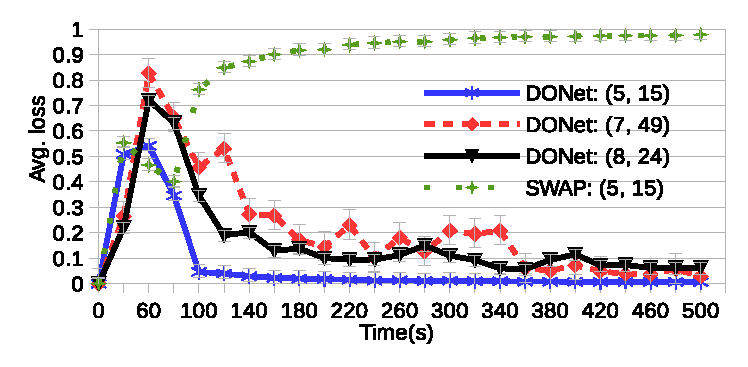
\includegraphics[width=8.4cm,height=3.5cm]{./Figures/avg-loss-donet.eps}}}
   \vspace{-1.5mm}
  \mbox{\subfloat[Avg. peer satisfaction]{\label{subfig:satisfaction-donet}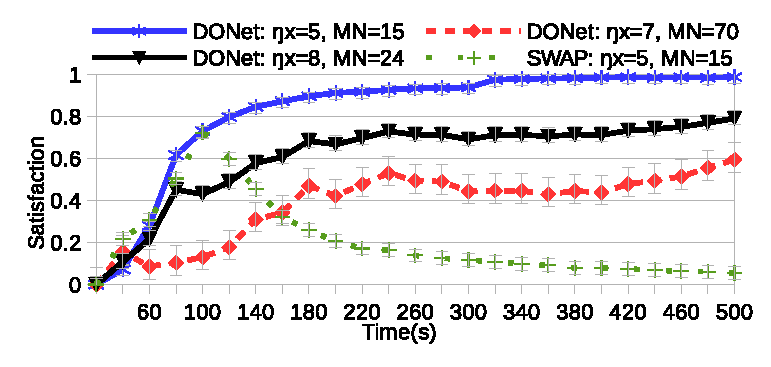
\includegraphics[width=8.4cm,height=3.5cm]{./Figures/satisfaction-donet.eps}}}
%   \mbox{\subfloat[Avg. loss]{\label{subfig:avg-loss-donet}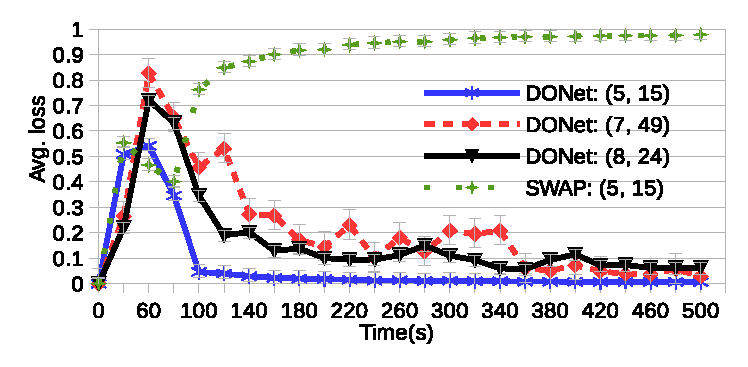
\includegraphics[width=3.7cm,height=2.5cm]{./Figures/avg-loss-donet.eps}} \subfloat[Avg. peer satisfaction]{\label{subfig:satisfaction-donet}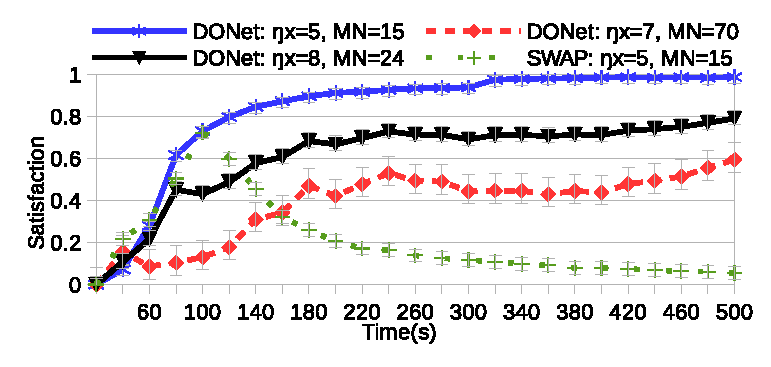
\includegraphics[width=3.7cm,height=2.5cm]{./Figures/satisfaction-donet.eps}}} 

  \caption{Attack's impact on DONet}
  \vspace{-3.5mm}
  \label{fig:attack-results}
  \end{figure}


\subsection{Case 2: Detection Mechanism Performance}

We now evaluate the performance of the detection mechanism.
Benign peers execute the detection mechanism as described in Section~\ref{sec:detection} whereas malicious peers aim to misuse the mechanism.
More precisely, malicious peers reply with a satisfaction level of 0 if the complaint might remove a benign peer and 1 if it might remove a malicious peer. 

In order to do so, we selected the following combinations for $(\eta x, MN)$: $(5, 80)$, $(8, 50)$ and $(10, 50)$ to assess the performance of the mechanism in severe attack conditions.
The satisfaction threshold $\satThres$ is set to 0.95 to measure if peers are able to fully restore their satisfaction level when the detection mechanism in operating.
The detection mechanism is effective starting $t=250s$ to allow for a reasonable amount of peers to join the overlay to adequately assess the efficiency of the mechanism.
In this scenario, every peer is allowed to initiate $\minDR=10$ detection requests for $t_{det}=500s$, and the minimum number of responses to generate a complaint is $\minP=3$. 
We discuss the effect of varying those parameters later on.

As depicted in Figure~\ref{subfig:BRNL}, once the detection mechanism is operating at $t=250s$, we observe an increase in the benign headnodes ratio in the source's neighbor list.
For instance, for $(\eta x, MN)=(5, 80)$, the source successfully attains ~80\% benign headnodes due to the detection mechanism.
For $(\eta x, MN)=(8, 50)$, the $BRNL$ ratio increases up to 90-100\%, which reflects the efficiency of the detection mechanism in replacing malicious headnodes to restore peers' satisfaction levels. 
Even if the source is initially only connected to malicious headnodes, i.e., $\eta x=10$, the detection mechanism is capable of restoring a $BRNL$ of close to 80\%. 

Figure~\ref{subfig:det-sat} illustrates the average restored peer satisfaction level due to the detection mechanism.
For the various attack placement strategies, the average satisfaction level increases up to ~95-100\%, even for $\eta x=10$.
As the detection mechanism starts at $t=250s$, the mechanism's impact on the peers satisfaction level $\sat$ can be noticed in a short time period.
The reason is that the number of initial detection requests sent to the source results in replacing a high fraction of the source's headnodes and quickly increases the satisfaction levels. 
Moreover, malicious peers are unable to misuse the detection mechanism, as indicated by the absence of degradation in  satisfaction levels. 

Figure~\ref{subfig:overhead} depicts the average detection overhead induced by our mechanism. 
As notice, the maximum overhead due to the detection mechanism is ~8\% for the different attack scenarios.
As peers are eventually satisfied, i.e., the number of detection requests initiated decreases, the overhead decreases to ~4\% at $t=500s$.
This implies that the overhead is not constant throughout time, i.e., once all peers' satisfaction level exceeds $\satThres$, they do not invoke the detection mechanism and hence do not induce additional overhead. 
Moreover, the maximum number of detection requests that can be initiated is dependent on $\minDR$, which is set to 10 in this scenario.
Thus, smaller values of $\minDR$ result in lower overhead, which is a useful application parameter that can be set according to suit the application's criticality or user's CPU resources.
In fact, varying $\minP$ between 3, 4 and 5 has little impact on the detection performance, indicating that nodes receive sufficient replies.

To that end, through the results, we highlight that the detection mechanism is indeed effective against \drop attacks, even if the attacker possesses high malicious budget as headnodes.
Moreover, we show that malicious peers are incapable of abusing the detection mechanism and place themselves as headnodes. Finally, the detection mechanism induces a very small overhead on the overlay.


\begin{figure}[t!]
\centering

  \mbox{\subfloat[Avg. BRNL]{\label{subfig:BRNL}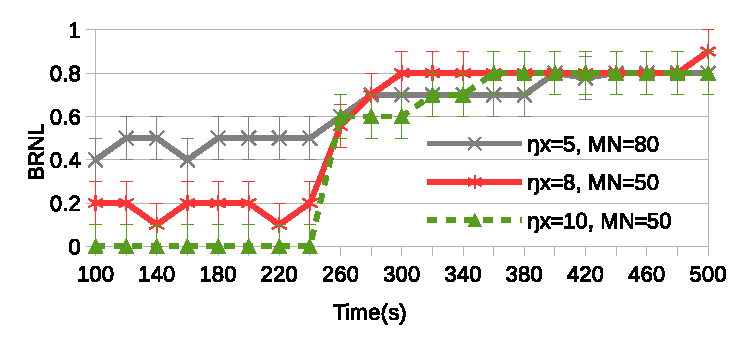
\includegraphics[width=8.4cm,height=3.5cm]{./Figures/det-BRNL1.eps}}}
\vspace{-1.5mm}    
  \mbox{\subfloat[Avg. peer satisfaction]{\label{subfig:det-sat}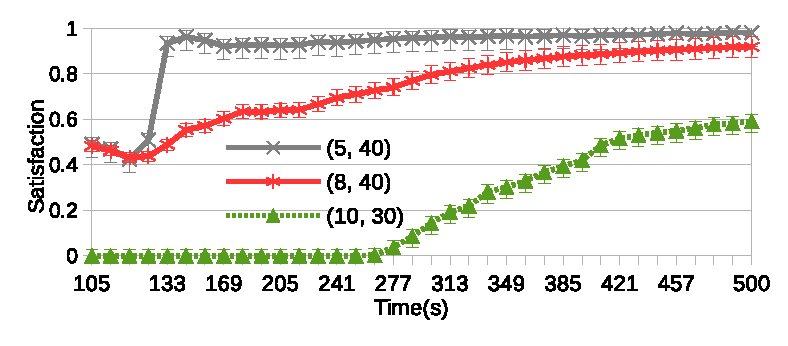
\includegraphics[width=8.4cm,height=3.5cm]{./Figures/det-sat.eps}}}
  \vspace{-1.5mm}   
   \mbox{\subfloat[Detection overhead]{\label{subfig:overhead}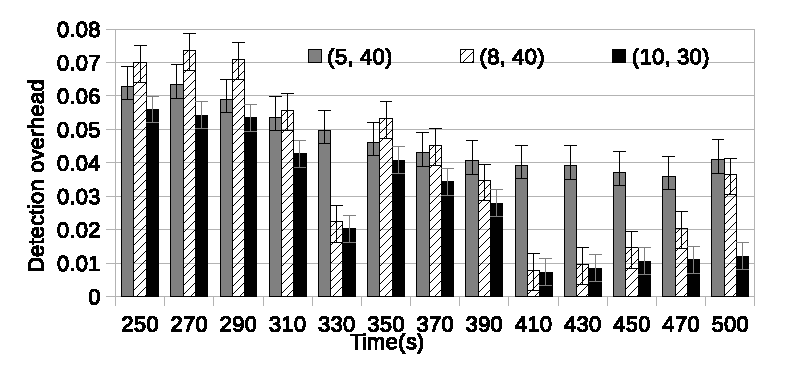
\includegraphics[width=8.4cm,height=3.5cm]{./Figures/overhead.eps}}}
%   \vspace{-1.5mm}   
%   \mbox{\subfloat[Avg. loss]{\label{subfig:avg-loss-donet}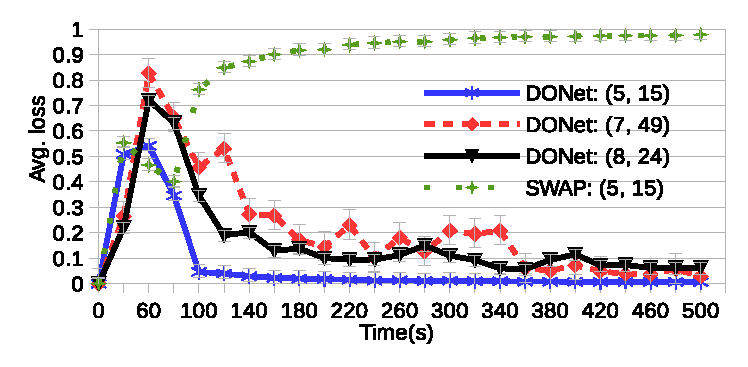
\includegraphics[width=3.7cm,height=2.5cm]{./Figures/avg-loss-donet.eps}} \subfloat[Avg. peer satisfaction]{\label{subfig:satisfaction-donet}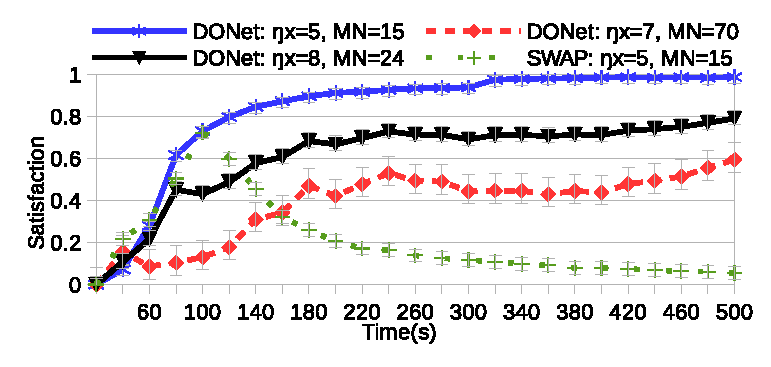
\includegraphics[width=3.7cm,height=2.5cm]{./Figures/satisfaction-donet.eps}}} 

  \caption{Detection mechanism performance}
  \vspace{-3.5mm}   
  \label{fig:detection-results}
  \end{figure}


% \subsubsection{Summary of the results}
% 
% As a summary, for DONet, when the source's neighbor list is fully saturated with malicious peers, $IL$ is at ~100\%.
% Nevertheless, for smaller values of $Hx$, the attack's impact is still significantly high for a long period of time given the intolerability of such networks to such high delays.
% In fact, having only $Hx=\alpha$ without using $MN$ is sufficient for the attacker to completely isolate and thus, prevent the source from delivering any stream chunks.
% 
% For the SWAP case study, it is noticed that even with low values of $Hx$, after a certain swapping period, malicious peers manage to fully occupy the source's list and hence, $IL$ eventually reaches to ~100\%.
% This denotes that, the number of neighbors $MN$ is a major factor in the case of SWAP.
% Moreover, through an efficient distribution of the attacker's budget $x$, i.e., $Hx$ and $MN$, the attacker can decide whether to cause higher damage to the stream at the initialization time and then allow the network to eventually recover later on, or to allow the stream to reach to benign peers at earlier time phase till totally cutting the flow once $Hx=\alpha$ at some point.


\section{Conclusion \& Future Work}
\label{sec:conclusion}
In this work\footnote{Research supported in part by EC H2020 CIPSEC GA \#700378 and BMBF TUD-CRISP}, we focus on the class of internal inference attacks for pull-based overlay where the attacker conducts a $BM$ cheating attack after placing malicious peers as headnodes.
We show that the attack severity increases the chunk loss ratio to ~10\%, accompanied by low satisfaction level experienced by benign peers.
As a countermeasure, we propose a detection mechanism where peers are able to collaboratively file a complaint to the source when their average aggregated satisfaction drops below a certain threshold so the source can replace suspicious headnodes.
% Accordingly, the source can replace specific headnodes that is most likely to be malicious.

Our simulations show that the detection mechanism is capable of restoring ~95-100\% of peers satisfaction level while removing ~80-90\% of malicious headnodes from its neighbor list while inducing a minimum overhead of approximately 8\%.
As an ongoing work, we focus on evaluating the resilience of our approach against various $BM$ cheating strategies and integrating anonymous monitoring for proactive defense.

 \bibliographystyle{unsrt}
 \bibliography{ref}

\IEEEpeerreviewmaketitle


\end{document}
	